\documentclass[10pt, a4paper]{amsart}

\usepackage{amsmath}
\usepackage{graphicx}
\usepackage{float}
\usepackage{caption}
\usepackage{subcaption}

\title{COMP0120 Project - Support Vector Machines (SVMs)}
\author{\textbf{John Duffy, Student Number: 19154676}}

\begin{document}

\maketitle

\section{Mathematical Setting - Summary}

\subsection{Binary Classification}\hfill

Primal Problem

\begin{figure}
	\centering	
	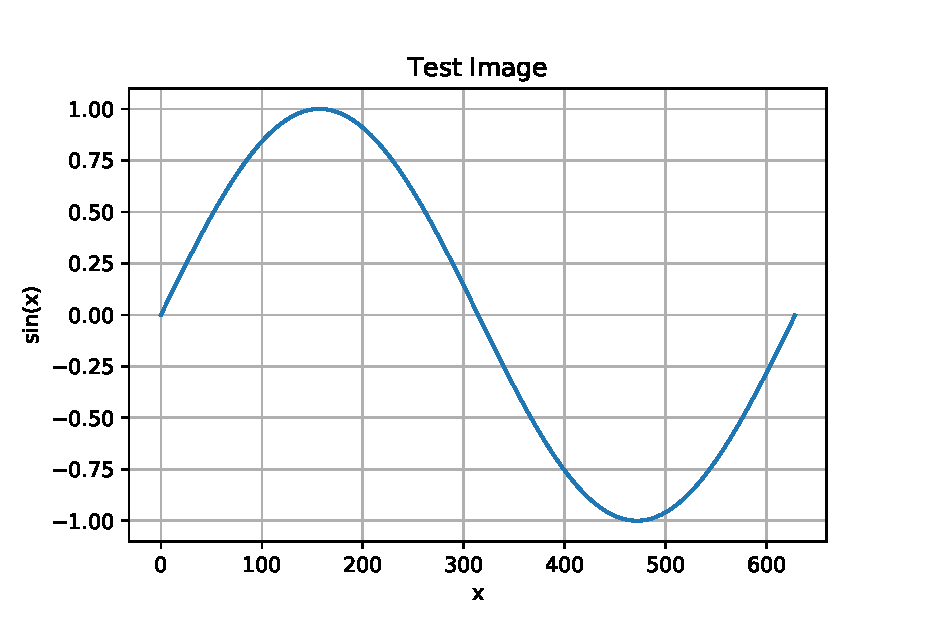
\includegraphics[width=1.0\textwidth]{test_image.eps}
	\caption{Image generation test from Jupyter Notebook.}
\end{figure}

\begin{figure}
	\centering	
	\begin{subfigure}{0.5\textwidth}
		\centering
		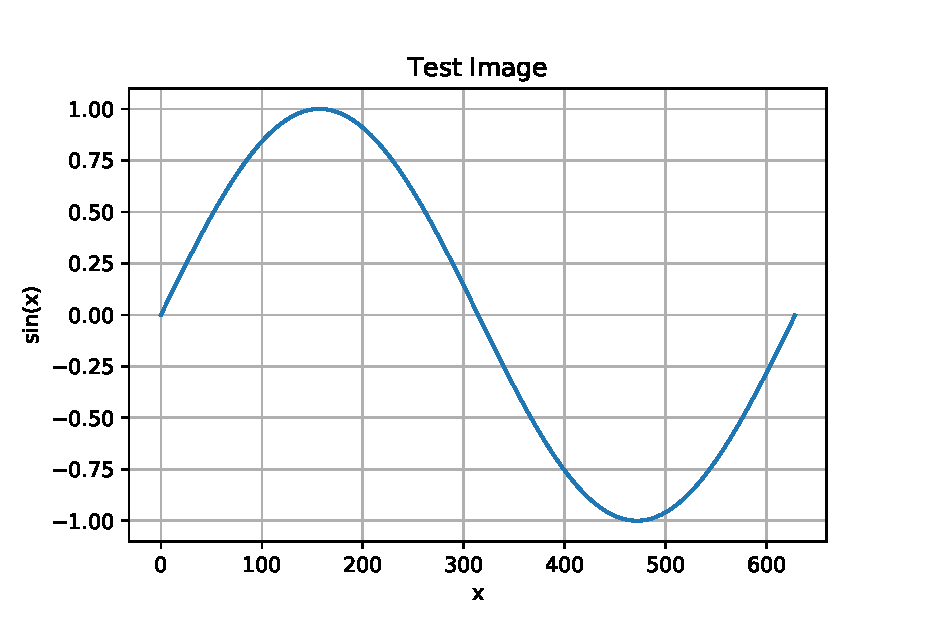
\includegraphics[width=1.0\textwidth]{test_image.eps}
		\caption{Image 1}
	\end{subfigure}%
	\begin{subfigure}{0.5\textwidth}
		\centering
		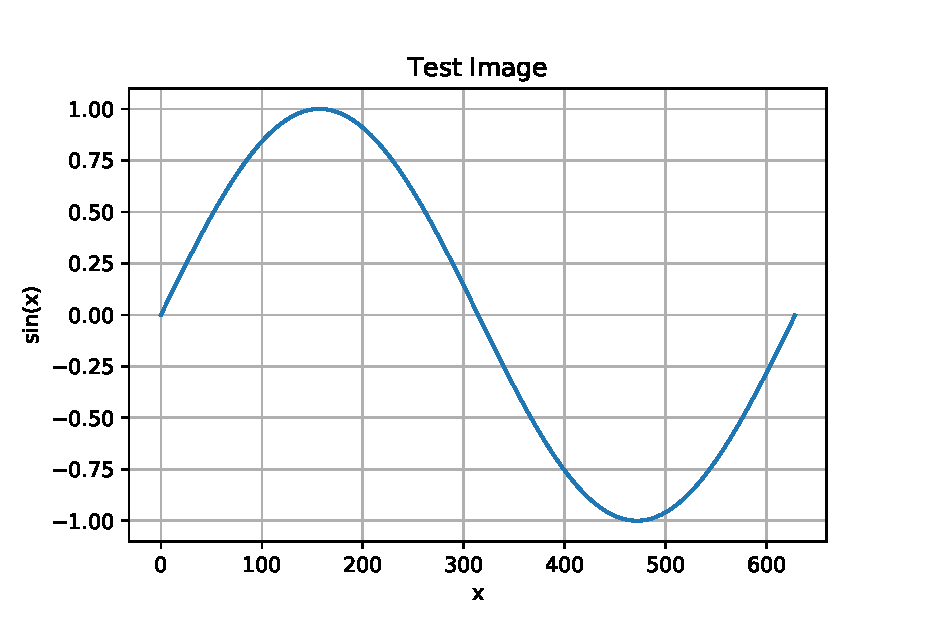
\includegraphics[width=1.0\textwidth]{test_image.eps}
		\caption{image 2}
	\end{subfigure}
	\caption{Image generation test from Jupyter Notebook.}
\end{figure}

Dual Problem

\subsection{Hard Margin}

\subsection{Soft Margin}

\subsection{Challenge!}\hfill

More classes?

Different Penalty Functions?

Algorithms not on syllabus?

\subsection{Non-Linear Classification}\hfill

Kernels?


\section{Simulation Study}

\subsection{Chosen Data Set}\hfill

Challenges?

How to address?

\subsection{Resulting Optimisation Problem}\hfill

Convex/Non-Convex

Constrained/Unconstrained

Smooth/Non-Smooth

Linear/Quadratic/Non-Linear

Challenges


\section{Solution of Optimisation Problem}

\subsection{Algorithm 1}\hfill

\subsection{Algorithm 2}\hfill


\section{References}

[1] ???

[2] ???

[3] ???

\end{document}
